\documentclass[11pt, oneside]{article} 
\usepackage{geometry}
\geometry{letterpaper} 
\usepackage{graphicx}
	
\usepackage{amssymb}
\usepackage{amsmath}
\usepackage{parskip}
\usepackage{color}
\usepackage{hyperref}

\graphicspath{{/Users/telliott/Github/calculus_book/png/}}
% \begin{center} 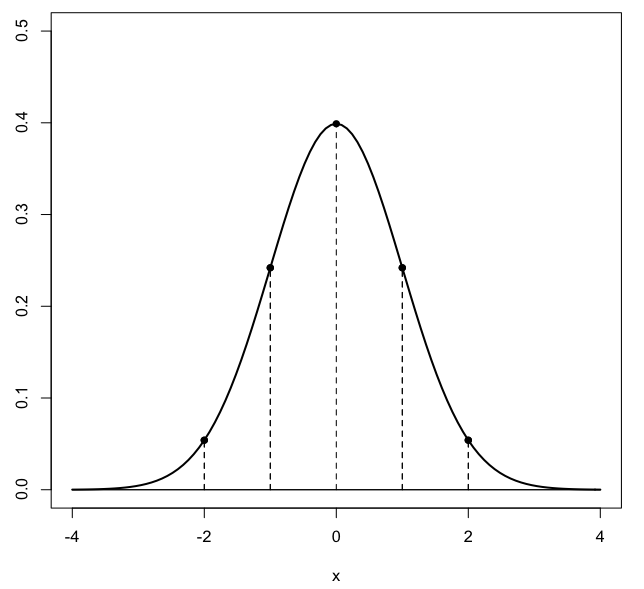
\includegraphics [scale=0.4] {gauss3.png} \end{center}

\title{Pythagorean Theorem}
\date{}

\begin{document}
\maketitle
\Large

\label{sec:pythagorean_thm}

The most famous theorem of Greek geometry is also the most useful in Calculus.  
\begin{center} 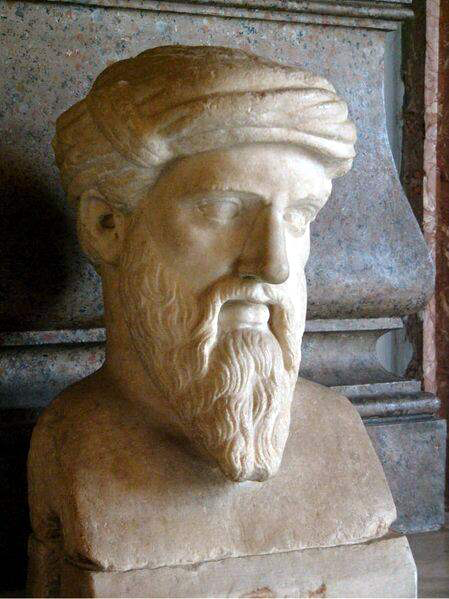
\includegraphics [scale=0.2] {pythagoras.png} \end{center}

Pythagoras (c.570-c.495 BC) was much younger than Thales but may have encountered him as a young man.  Like many other Greek mathematicians, Pythagoras was not from the mainland, but from one of the islands, in his case, Samos, which is not far from Miletus, where Thales lived.  

Pythagoras was famous as a philosopher as well as a mathematician.  In fact, he founded a famous "school" and it is not sure now which of the theorems developed by this school are due to Pythagoras, and which to his disciples.  It is not even clear whether the Pythagorean theorem, as we know it, was known to Pythagoras.

However, it's pretty certain that they knew something.  The $3,4,5$ right triangle and many other Pythagorean triples (see below) had been known for a thousand years (since 1500 BC).  Here is a special case, easily proved, for an isosceles right triangle.

\begin{center} 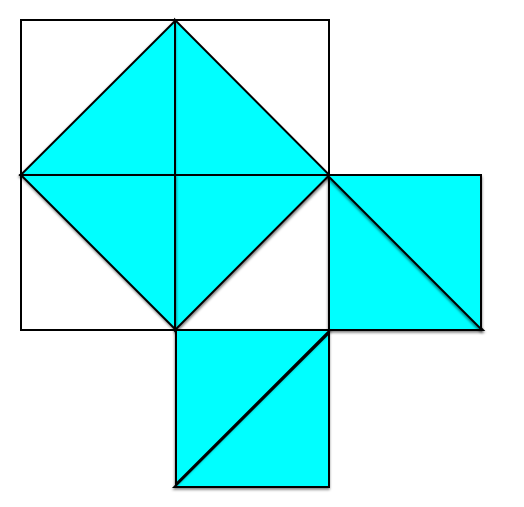
\includegraphics [scale=0.3] {pyth7.png} \end{center}

The area of the square on the hypotenuse is equal to twice the area on each side.

There are literally hundreds of proofs of the general theorem, that if $a$ and $b$ are the shorter sides of a right triangle and $c$ is the hypotenuse, then
\[ a^2 + b^2 = c^2 \]

This one is sometimes called the "Chinese proof."  I can easily imagine proceeding from the figure above to this one by simply rotating the inner square.

\begin{center} 
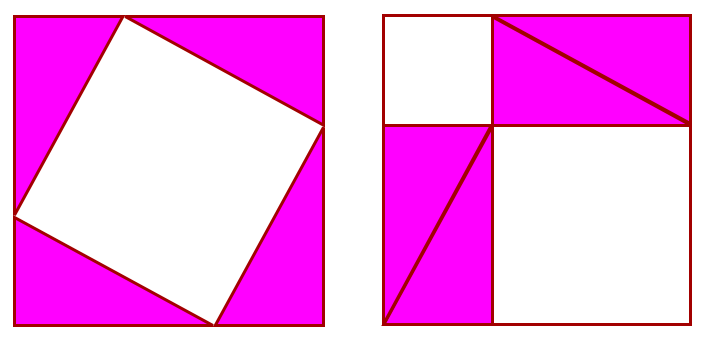
\includegraphics [scale=0.25] {pythagoras1.png} 
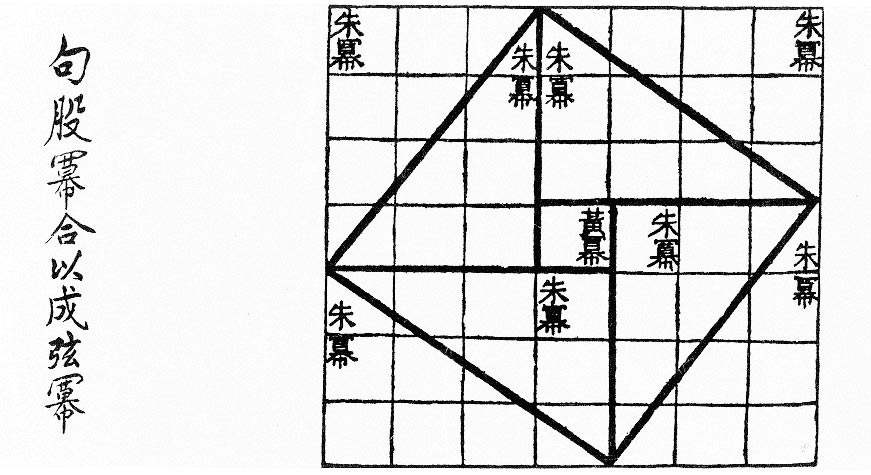
\includegraphics [scale=0.25] {Chinese_pythagoras.jpg}
\end{center}

It really needs no explanation, but ..

In the left panel we have a large square box that contains within it a white square, whose side is also the hypotenuse of the four identical right triangles contained inside.  Altogether the four triangles plus the white area add up to the total.

We simply rearrange the triangles.  Now we evidently have the same area left over from the four triangles, because they still have the same area and the surrounding box has not changed.  

But clearly, now the white area is the sum of the squares on the second and third sides of the triangles.  Hence the two white squares on the right are equal in area to the large white square on the left.  $\square$

This proof is contained in the Chinese text Zhoubi Suanjing (right panel, above).

\url{https://en.wikipedia.org/wiki/Zhoubi_Suanjing}

\subsection*{Euclid's proof}
\begin{center} 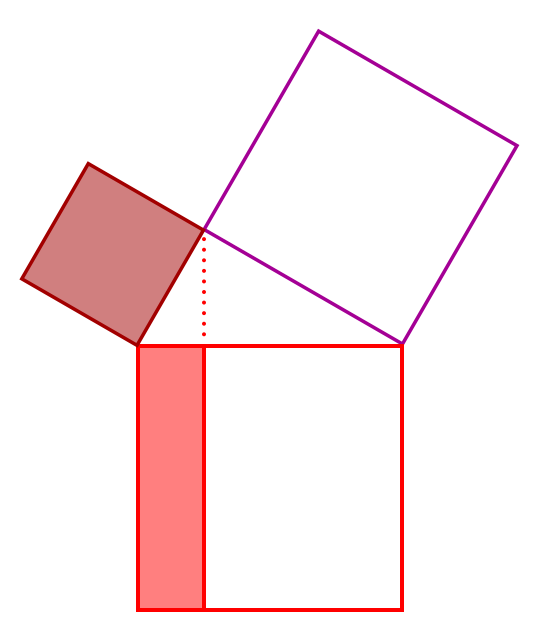
\includegraphics [scale=0.3] {pythagoras2.png} \end{center}

My favorite proof relies on the construction above (Euclid $I.47$, sometimes called the "bridal chair" or the "windmill"), where the central triangle is a right triangle, and the other constructions are squares.  It is a bit more detailed, but it is  one of only a few places in the book that we actually show a proof from Euclid, which is a justification for including it.

What we will show is that the part of the large square in red is equal in area to the entire small square, in maroon.

We label some points as shown:
\begin{center} 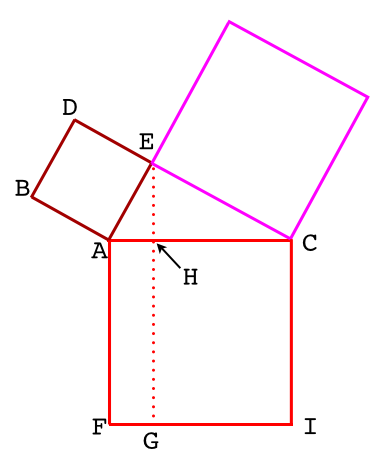
\includegraphics [scale=0.45] {pythagoras3.png} \end{center}
   
First, drop a vertical line $EHG$, constructing the rectangle $AFGH$.
   
Finally, sketch dotted lines for the long sides of two triangles:
\begin{center} 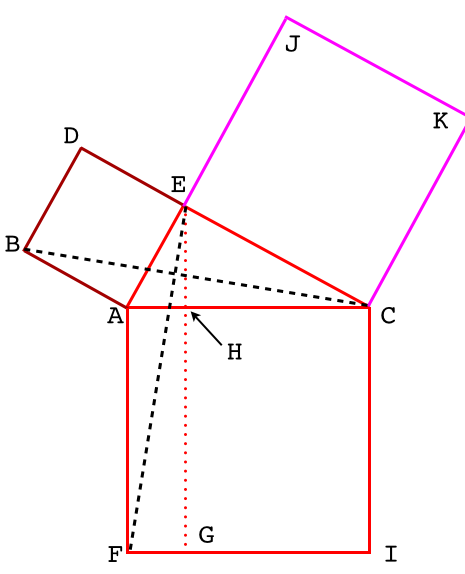
\includegraphics [scale=0.4] {pythagoras4.png} \end{center}

The crucial point is this:  we will show that triangle $\Delta ABC$ is congruent to triangle $\Delta AEF$.  

Use "side-angle-side".  The two sets of sides are evidently equal 
\[ AB = AE, \ \ \ \ AC = AF \]
because these are given as sides of two squares.

What about the included angle?  Both angle $\angle BAC$ and $\angle EAF$ contain a right angle plus the shared angle $\angle EAC$.  So they are themselves equal, and thus we have proved the congruence relationship:
\[ \Delta ABC = \Delta AEF \]

The next part of the proof is to tilt triangle $\Delta ABC$ to the left and see that it has base $AB$ and altitude $AE$ so its area is one-half that of the small square $ABDE$.  On the other hand triangle $\Delta AEF$ has base $AF$ and altitude $AH$ (as well as $FG$) so its area is one-half that of the rectangle $AFGH$.

Hence we have proved that the two colored areas in this figure are equal:

\begin{center} 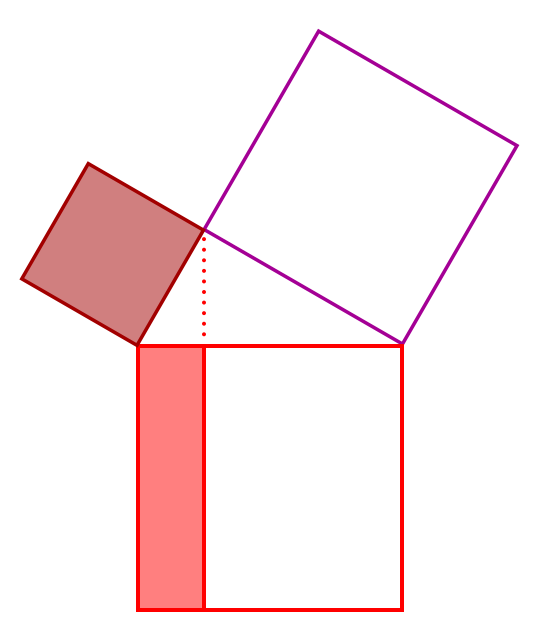
\includegraphics [scale=0.35] {pythagoras2.png} \end{center}
Finally, we could proceed to do the same thing on the right side of the figure, but we just appeal to symmetry.  All the equivalent relationships will hold.  $\square$

\subsection*{algebraic proofs}

The following proofs are algebraic ones.  Not so pretty, but fast.  

Arrange 4 identical right triangles as shown in the figure below.  The four triangles plus a small central square form a larger quadrilateral which is also a square.

\begin{center} 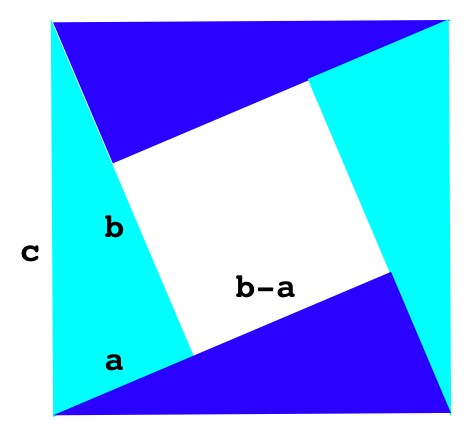
\includegraphics [scale=0.4] {pythagoras5.png} \end{center}

The angles at the corners of the quadrilateral, at the points flanking the hypotenuse $c$, are right angles, because they are formed by addition of two complementary angles of congruent right triangles.  Since the quadrilateral has four internal right angles and equal length sides, it is a square.

Now just calculate the area of the parts.  We have four identical right triangles with sides $a$ and $b$, plus the central square with sides $b-a$.  The area is 
\[ A = 4 \cdot \frac{1}{2}ab + (b - a)^2 \]
\[ = b^2 + a^2 \]

But the area is also the square of side $c$.  

$\square$

We have used various properties proved earlier, e.g. that the sum of the angles of any triangle is $180$ degrees.

Here is a very similar proof:

\begin{center} 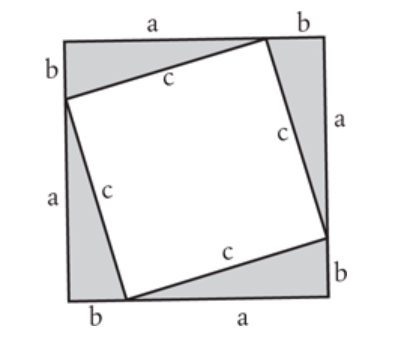
\includegraphics [scale=0.5] {pythagoras6.png} \end{center}

In this figure, the right triangles are aligned so that the big square has sides which combine the lengths $a + b$ and have area $(a + b)^2$.  But we can also calculate the area as the sum of its components, namely, central tilted square plus the four triangles:

\[ (a + b)^2 = c^2 + 4 \cdot \frac{ab}{2} \]
\[ a^2 + b^2 + 2ab =  c^2 + 2ab \]
\[ a^2 + b^2 = c^2 \]

$\square$

For the third algebraic proof, divide a right triangle into two smaller ones by dropping an altitude, which meets the base at a right angle.
\begin{center} \includegraphics [scale=0.5] {triangle.png} \end{center}

By complementary angles, these three triangles are all similar (e.g., the angle between sides $b$ and $h$ is equal to that between sides $a$ and $c$).  So we can construct ratios of sides that are equal.

We need a relationship involving $a^2$.
\[ \frac{h}{b} = \frac{e}{a} = \frac{a}{c} \]
We choose the ones involving $c$ and $e$:
\[ a^2 = ce \]
\begin{center} \includegraphics [scale=0.5] {triangle.png} \end{center}

and also a relationship involving $b^2$:

\[  \frac{b}{d} = \frac{c}{b}  \]
\[  b^2 = cd  \]

Putting the two together:
\[ a^2 + b^2 = ce + cd \]
\[ = c (d+e) = c^2 \]

Which is what we wanted to prove.  $\square$

There are more than 300 proofs of this theorem, including one by a President of the United States, James A. Garfield.  

Here is his proof:
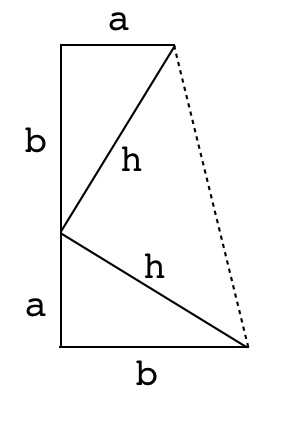
\includegraphics [scale=0.4] {garfield.png}
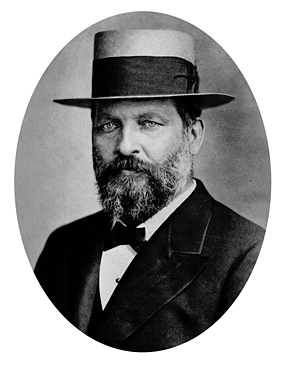
\includegraphics [scale=0.4] {garfield2.png}

Draw a right triangle and a rotated copy as shown.  The area of the quadrilateral is the product of the side $(a + b)$ and the \emph{average} of $a$ and $b$:
\[ A = (a+b) \cdot \frac{1}{2} (a + b) \]
If you don't see this right away, calculate the area as a rectangle plus a triangle (whose side is not shown but drops vertically from the top right corner).
\[ a(a + b) + \frac{1}{2}(b-a)(a+b) \]
with the same result so
\[ A = \frac{1}{2} a^2 + ab + \frac{1}{2} b^2 \]
But it is also the sum of 
\[ \frac{1}{2} ab + \frac{1}{2} ab + \frac{1}{2} h^2 \]
Equate the two and the result follows almost immediately.

$\square$

\subsection*{Corollary}
There are several important corollaries of the Pythagorean theorem.  We'll derive one later called the law of cosines.  Here is another from the Islamic geometer Ibn Quorra, who brought algebraic techniques, shunned by the Greeks, to geometry.
\begin{center} 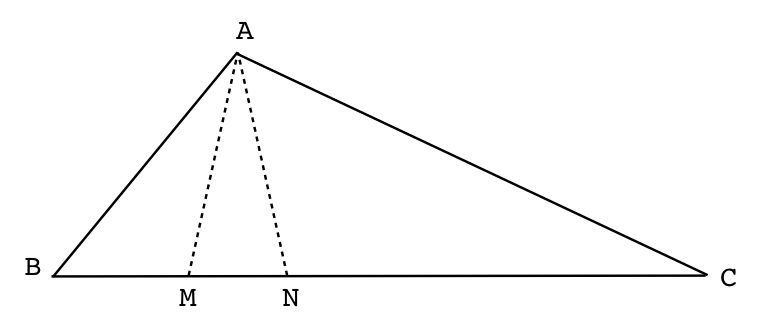
\includegraphics [scale=0.4] {pyth_corollary.png} \end{center}

Let $\triangle ABC$ be \emph{any} triangle (here it is obtuse).  Draw $AM$ and $AN$ so that the new angles $\angle AMB$ and $\angle ANC$ are equal to $\angle A$.  The corresponding triangles are similar to the original, because they share the angle of measure $A$ plus one other from the original triangle.

Then
\[ BM:AB = AB:BC \]
Thus, $AB^2 = BM \times BC$.  Similarly
\[ NC:AC = AC:BC  \]
So $AC^2 = NC \times BC$
Therefore
\[ AB^2 + AC^2 = BM \times BC + NC \times BC \]
\[ = (BM + NC) \times BC \]

In the case where the angle at vertex $A$ is a right angle, then $M$ coincides with $N$, and $BM + NC = AC$, and this reduces to the Pythagorean theorem.

\subsection*{Pythagorean triples}
The simplest right triangle with integer sides is $3,4,5$:
\[ 3^2 + 4^2 = 5^2 \]

any multiple $n$ will work
\[ (3n)^2 + (4n)^2 = (5n)^2 \]
but that's not so interesting.  The triples which are not multiples of another triple are called \emph{primitive}.

To go further, we can use Euclid's formula.  For every integer $m,n$, with $m > n$, a Pythagorean triple is given by
\[ a = m^2 - n^2 \ \ \ \ b = 2mn \ \ \ \ c = m^2 + n^2 \]

It is better to choose $m$ and $n$ of opposite parity (one even and one odd).  Otherwise, $a$, $b$ and $c$ will all be even and the triple won't  be primitive.

It is easy to see why this works:
\[ a^2 + b^2 = (m^2 - n^2)^2 + (2mn)^2 \]
\[ = m^4 - 2m^2n^2 + n^4 + 4m^2n^2 \]
\[ = m^4 + 2m^2n^2 + n^4 \]
\[ = (m^2 + n^2)^2 = c^2 \]

Suppose $a = 5$.  The two squares with a difference of $5$ are 
\[ 3^2 - 2^2 = 5 \]
So $b = 2mn = 12$ and $c = 3^2 + 2^2 = 13$.  And indeed $5^2 + 12^2 = 13^2$.

\url{https://en.wikipedia.org/wiki/Pythagorean_triple#Enumeration_of_primitive_Pythagorean_triples}

A thousand years before Pythagoras, the Babylonians knew the triple $4601,4800,6649$.  It seems unlikely that they found this by random search.

\subsection*{geometric mean}

As a slight detour from calculus, but on the topic of this chapter

\begin{center} 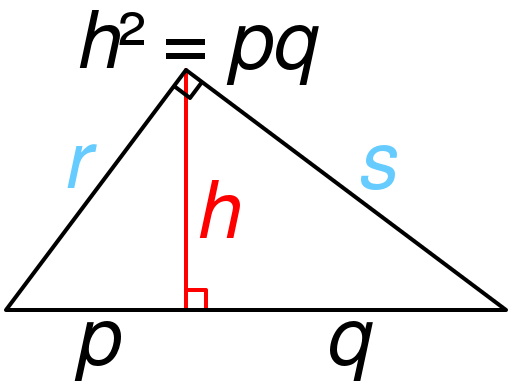
\includegraphics [scale=0.25] {geometric_mean.png} \end{center}

According to the figure, the altitude of a right triangle is related to the two segments along the base by
\[ h^2 = pq \]
\[ h = \sqrt{pq} \]
That is, $h$ is the geometric mean of these two values $p$ and $q$.

The proof is simple.  Using the Pythagorean theorem with the two small triangles (also right triangles), we obtain:
\[ h^2 + p^2 = r^2 \]
\[ h^2 + q^2 = s^2 \]
Summing
\[ 2h^2 + p^2 + q^2 = r^2 + s^2 \]

Using the theorem with the big triangle:
\[ r^2 + s^2 = (p + q)^2 \]
\[ = p^2 + 2pq + q^2 \]

Equating the two expressions for $r^2 + s^2$ we get:
\[ 2h^2 + p^2 + q^2 = p^2 + 2pq + q^2 \]
\[ h^2 = pq \]

According to wikipedia:

\url{https://en.wikipedia.org/wiki/Geometric_mean}

The fundamental property of the geometric mean is that (letting $m$ be the \emph{geometric mean} here):
\[ m \ [ \ \frac{x_i}{y_i} \ ] \ = \frac{m(x_i)}{m(y_i)} \]

and one consequence is that

\begin{quote}This makes the geometric mean the only correct mean when averaging normalized results; that is, results that are presented as ratios to reference values.\end{quote}

A number of examples are given in the article.

Last:  a proof-without-words that the geometric mean is always less than or equal to the arithmetic mean.

\begin{center} 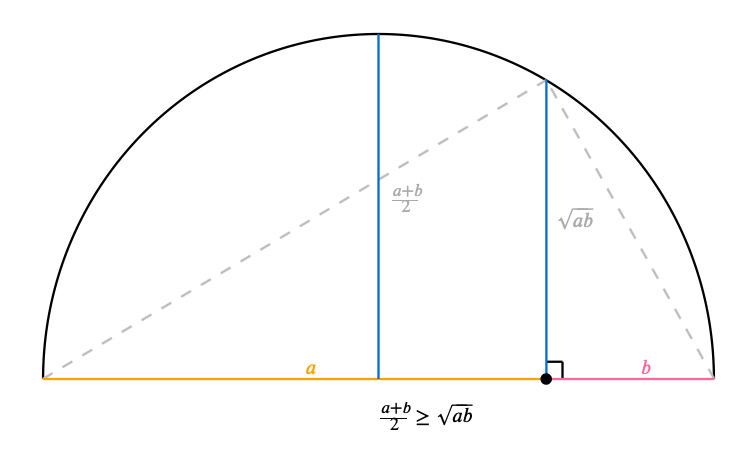
\includegraphics [scale=0.4] {pww_geomean.png} \end{center}

 
\end{document}